\section{Anexos de la Práctica 5}


\begin{figure}[ht!] % 'h' indica que la imagen se coloca aquí
    \centering
    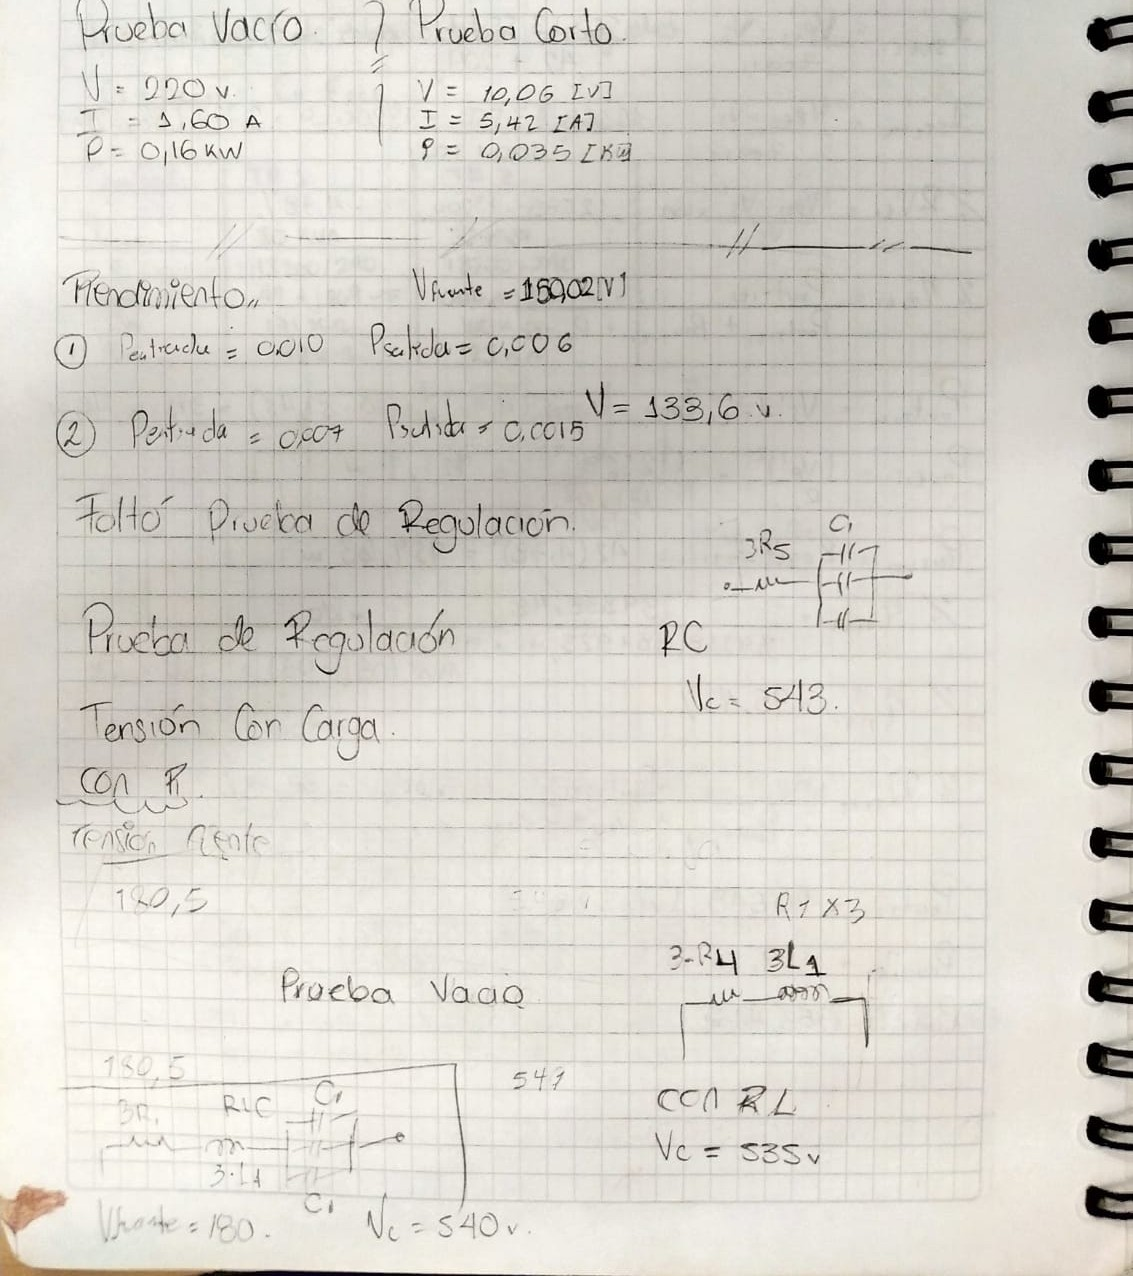
\includegraphics[width=0.48\textwidth]{fot/prac4_hoja de tales.jpg} % Cambia la ruta a tu imagen
    \caption{Hoja de la practica con los resultados de las pruebas.}
    \label{fig:hoja}
\end{figure}


\begin{figure}[ht!] % 'h' indica que la imagen se coloca aquí
    \centering % Centra la imagen
    \begin{subfigure}{0.5\textwidth}
            \centering
            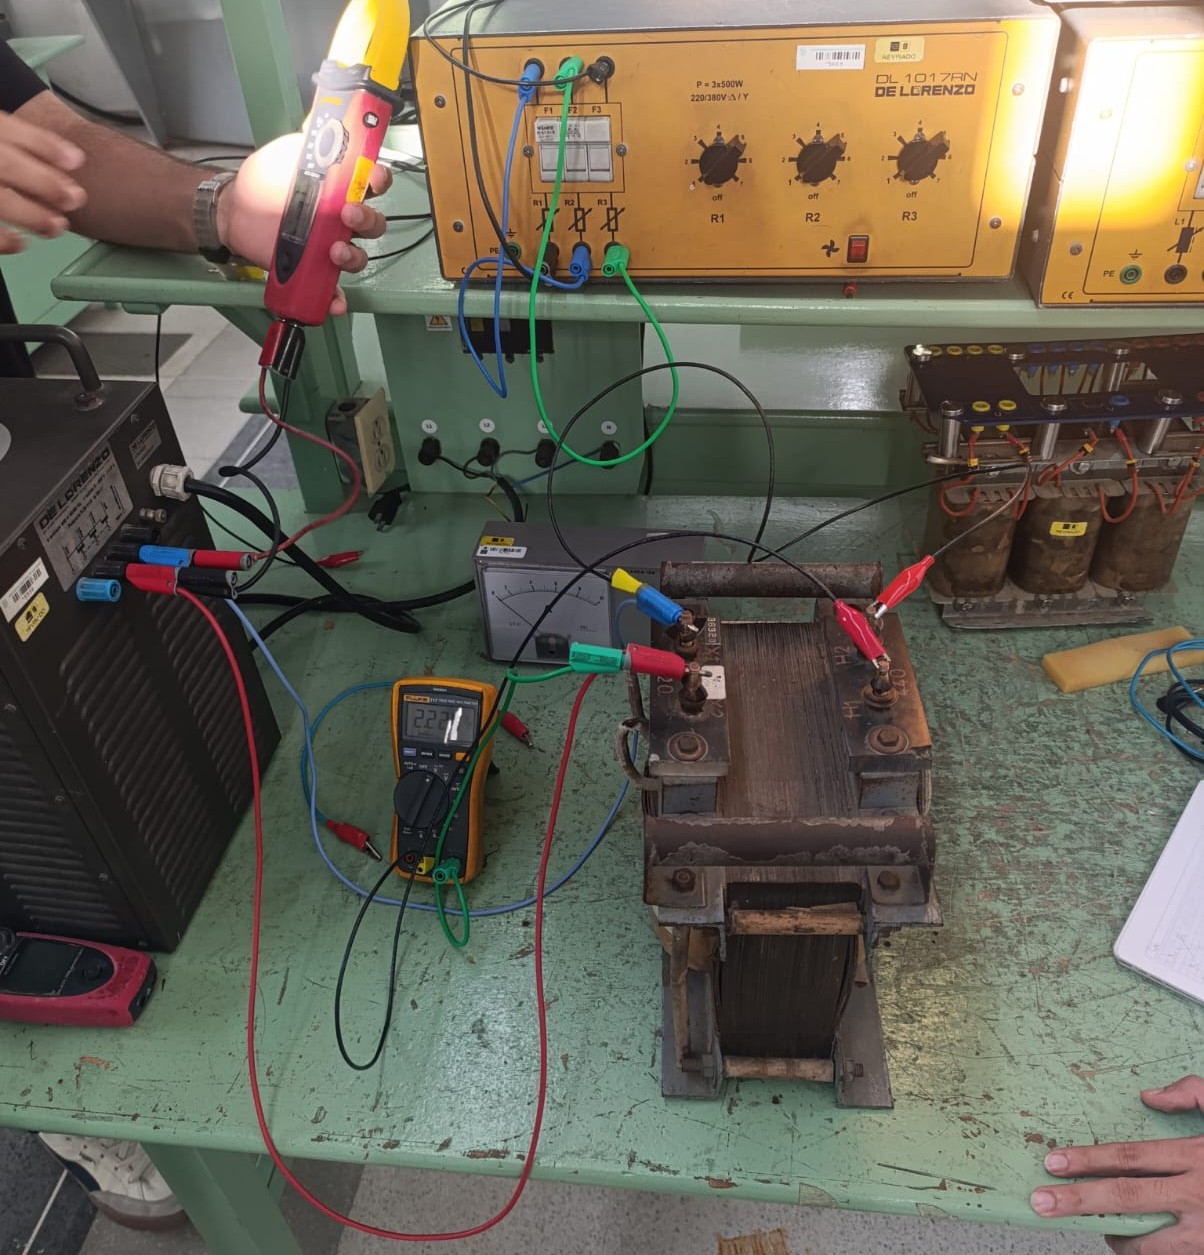
\includegraphics[width=0.8\textwidth]{fot/prac4_autoenvacio.jpeg} % Cambia la ruta a tu imagen
            \caption{Autotransformador en la prueba de vacio (Hay una carga de resistencias en serie que estan desconectadas).}
            \label{fig:prac4_autoenvacio}
    \end{subfigure}
    \hfill % Espacio horizontal entre las subfiguras
    \begin{subfigure}{0.5\textwidth}
        \centering
        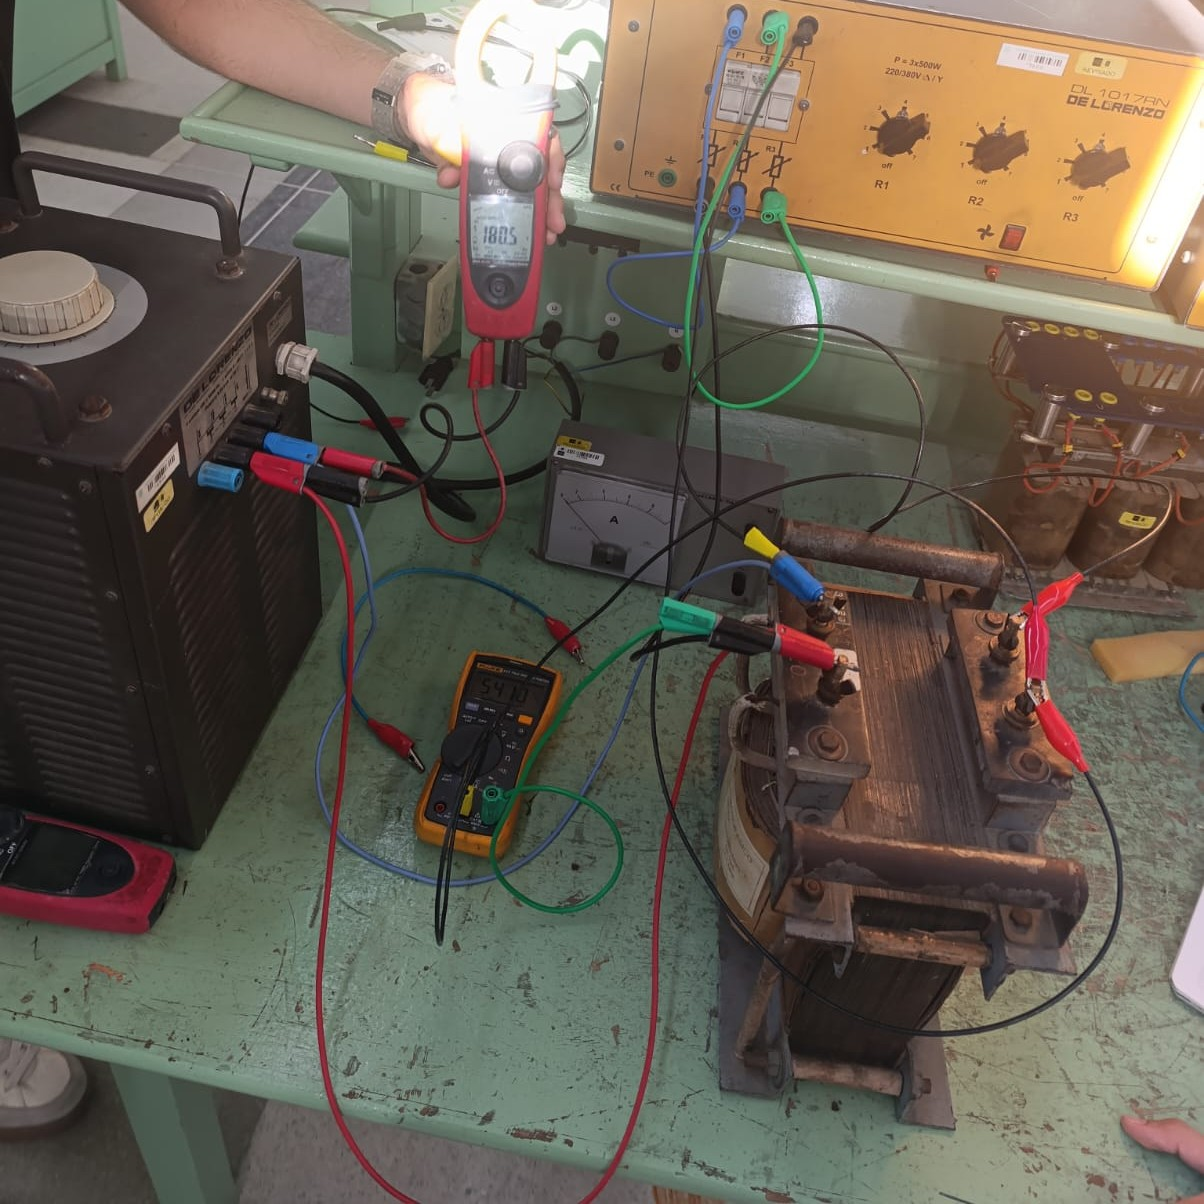
\includegraphics[width=0.8\textwidth]{fot/prac4_autoR_.jpeg} % Cambia la ruta a tu imagen
        \caption{Autotransformador con tres cargas resistivas conectadas en serie.}
        \label{fig:AutoR1}  
    \end{subfigure}
    \label{fig:dos-imagenes}
    \hfill
    \begin{subfigure}{0.5\textwidth} % Corrected missing curly brace
        \centering
        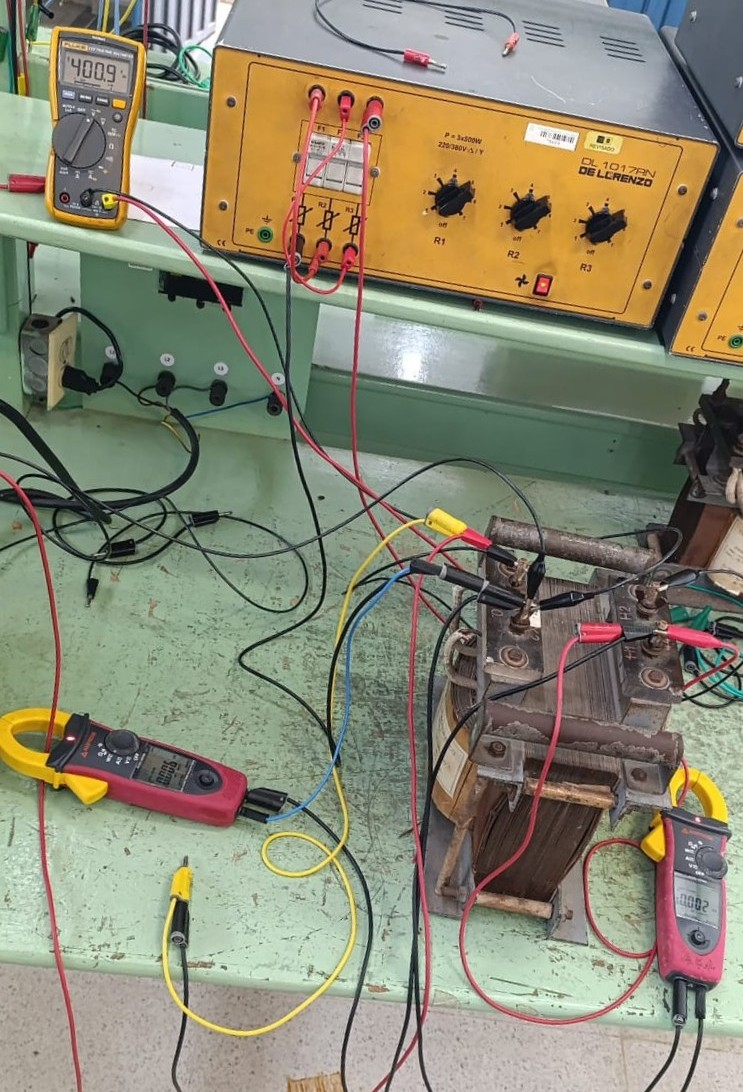
\includegraphics[width=0.8\textwidth]{fot/prac4_rendimiento.jpg} % Cambia la ruta a tu imagen
        \caption{Autotransformador realizando prueba de rendimiento.}
        \label{fig:Autorendimiento}
    \end{subfigure}
\end{figure}